%%%%%%%%%%%%%%%%%%%%%%%%%%%%%%%%%%%%%%%%%
% University/School Laboratory Report
% LaTeX Template
% Version 3.1 (25/3/14)
%
% This template has been downloaded from:
% http://www.LaTeXTemplates.com
%
% Original author:
% Linux and Unix Users Group at Virginia Tech Wiki 
% (https://vtluug.org/wiki/Example_LaTeX_chem_lab_report)
%
% License:
% CC BY-NC-SA 3.0 (http://creativecommons.org/licenses/by-nc-sa/3.0/)
%
%%%%%%%%%%%%%%%%%%%%%%%%%%%%%%%%%%%%%%%%%

%----------------------------------------------------------------------------------------
%	PACKAGES AND DOCUMENT CONFIGURATIONS
%----------------------------------------------------------------------------------------

\documentclass{article}

\usepackage[version=3]{mhchem} % Package for chemical equation typesetting
\usepackage{siunitx} % Provides the \SI{}{} and \si{} command for typesetting SI units
\usepackage{graphicx} % Required for the inclusion of images
\usepackage{natbib} % Required to change bibliography style to APA
\usepackage{amsmath} % Required for some math elements 
\usepackage{caption}
\usepackage{subcaption}

\setlength\parindent{0pt} % Removes all indentation from paragraphs

\renewcommand{\labelenumi}{\alph{enumi}.} % Make numbering in the enumerate environment by letter rather than number (e.g. section 6)

%\usepackage{times} % Uncomment to use the Times New Roman font

%----------------------------------------------------------------------------------------
%	DOCUMENT INFORMATION
%----------------------------------------------------------------------------------------

\title{COMP 429/529: Project 1} % Title

\author{Berkay \textsc{Barlas}} % Author name

\date{\today} % Date for the report

\begin{document}

\maketitle % Insert the title, author and date

\begin{center}
\begin{tabular}{l r}
Date Performed: & March 17, 2019 \\ % Date the experiment was performed
Instructor: & Didem Unat % Instructor/supervisor
\end{tabular}
\end{center}

% If you wish to include an abstract, uncomment the lines below
% \begin{abstract}
% Abstract text
% \end{abstract}

%----------------------------------------------------------------------------------------
%	SECTION 1
%----------------------------------------------------------------------------------------

\section{Part I: Image Blurring}

To determine the atomic weight of magnesium via its reaction with oxygen and to study the stoichiometry of the reaction (as defined in \ref{definitions}):

%\begin{center}\ce{2 Mg + O2 -> 2 MgO}\end{center}

% If you have more than one objective, uncomment the below:
%\begin{description}
%\item[First Objective] \hfill \\
%Objective 1 text
%\item[Second Objective] \hfill \\
%Objective 2 text
%\end{description}

\subsection{Stability Test}

\begin{description}
    \item[Serial version execution time: ] 
    \item[Paralel version with single thread execution time: ]
    The
    \item[Which thread number gives best performance?]
    32 thread count gives best performance for both blurring applications.
\end{description}

Results

\begin{figure}[!htb]
    \centering
    \begin{subfigure}{.45\textwidth}
        \centering
        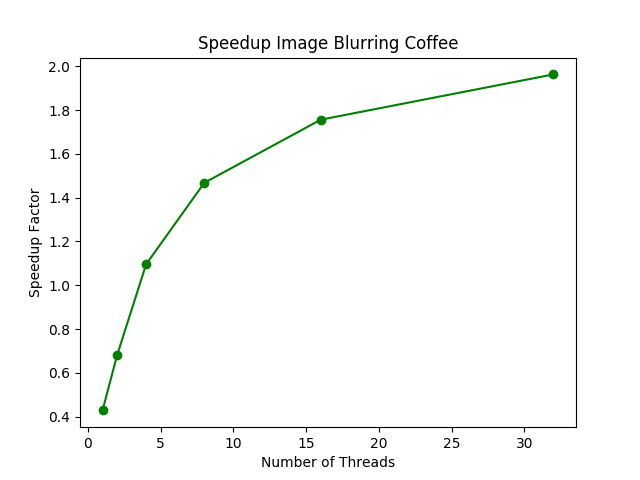
\includegraphics[width=1\linewidth]{./img/speedup_part_1_A.png}
        \caption{Results for the blurring on coffee image.}
    \end{subfigure} 
    \begin{subfigure}{.45\textwidth}
        \centering
        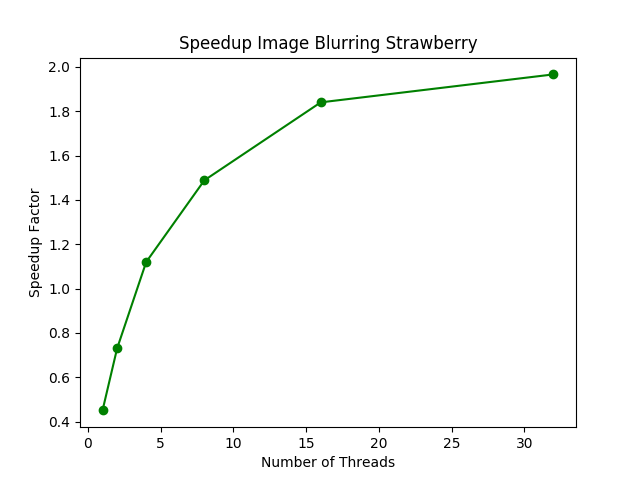
\includegraphics[width=1\linewidth]{./img/speedup_part_1_A_strawberry.png}
        \caption{Results for the blurring on strawberry image.}
    \end{subfigure}
    \caption{Speedup figures for image blurring application}
\end{figure}   

EXPLAIN SPEEDUP CURVE
\newline
asfsadfasdf
sadf
fasdfasdfa
\newpage

\subsection{Thread Binding Test}
a
\begin{description}
    \item[Different mapping strategies; Compact and Scatter]
\end{description}
 Results 
 \begin{figure}[!htb]
    \centering
    \begin{subfigure}{.45\textwidth}
        \centering
        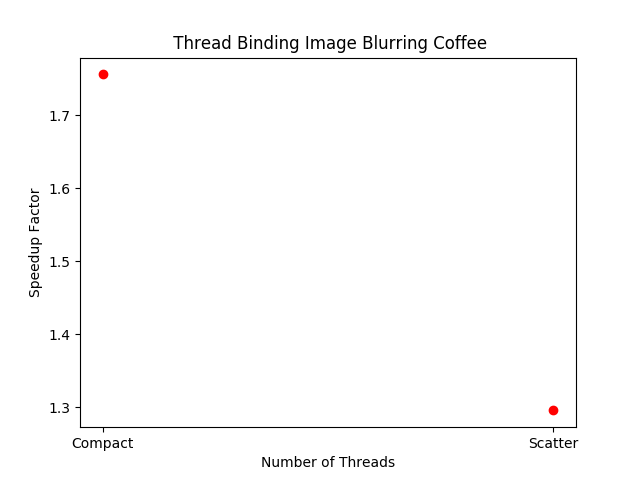
\includegraphics[width=1\linewidth]{./img/binding_part_1_B_coffee.png}
        \caption{Results for the blurring on coffee image.}
    \end{subfigure} 
    \begin{subfigure}{.45\textwidth}
        \centering
        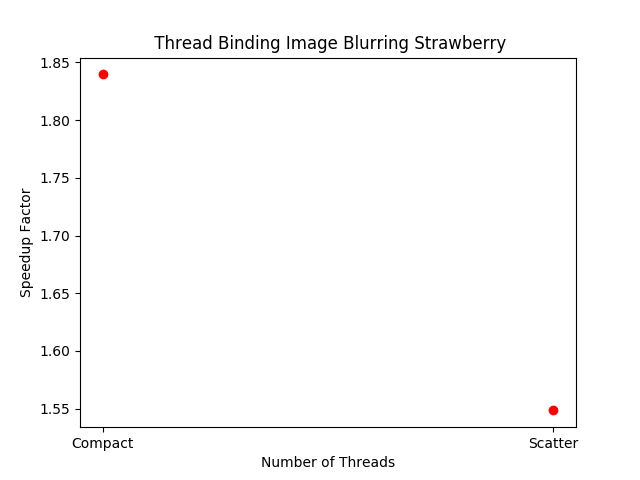
\includegraphics[width=1\linewidth]{./img/binding_part_1_B_strawberry.png}
        \caption{Results for the blurring on strawberry image.}
    \end{subfigure}
    \caption{Speedup figures for image blurring application}
\end{figure}

WHICH MAPPING GIVES BETTER PERFORMANCE, WHY ? 

%----------------------------------------------------------------------------------------
%	SECTION 2
%----------------------------------------------------------------------------------------
\newpage

\section{PART II: Parallel Sudoku Solver}

\begin{tabular}{ll}
Mass of empty crucible \\

\end{tabular}

\subsection{Scalability Test}
\subsubsection{Part A}
\begin{description}
\item[Serial version execution time: ] 
\item[Paralel version with single thread execution time: ]
\item[Which thread number gives best performance?]
The
\end{description} 

Results 
 \begin{figure}[!htb]
    \centering
        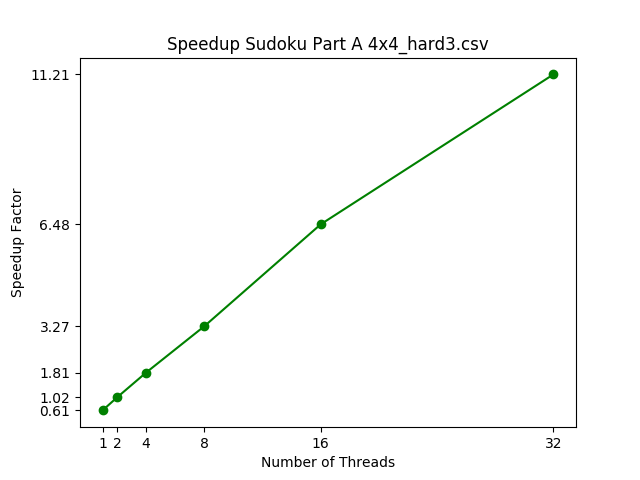
\includegraphics[width=1\linewidth]{./img/speedup_part_2_A.png}
        \caption{\small Results for the Sudoku 4x4hard3 using algorithm in.}
\end{figure}                

\newpage

\subsubsection{Part B}
\begin{description}
\item[Serial version execution time: ] 
\item[Paralel version with single thread execution time: ]
\item[Which thread number gives best performance?]
The
\end{description} 
\begin{figure}[!htb]
        \centering
        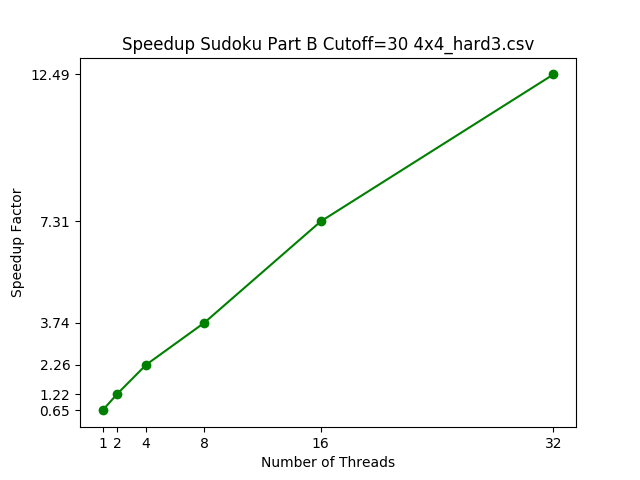
\includegraphics[width=1\linewidth]{./img/speedup_part_2_B.png}
        \caption{Results for the blurring on strawberry image.}
\end{figure}

\newpage

\subsubsection{Part C}
\begin{description}
\item[Serial version execution time: ] 
\item[Paralel version with single thread execution time: ]
\item[Which thread number gives best performance?]
The
\end{description} 

\begin{figure}[!htb]
        \centering
        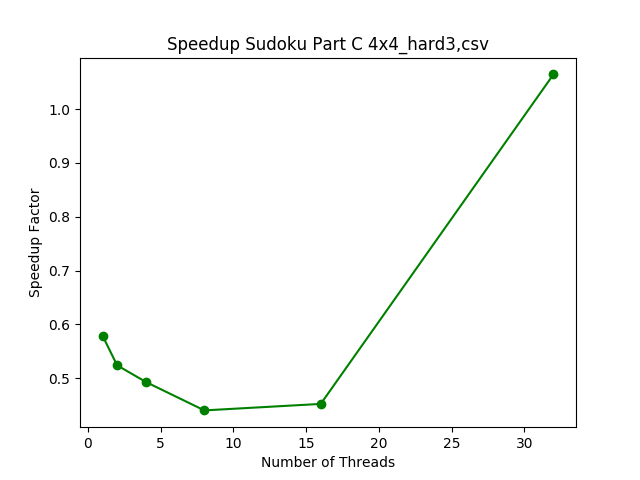
\includegraphics[width=1\linewidth]{./img/speedup_part_2_C.png}
        \caption{Results for the blurring on strawberry image.}
\end{figure}
    
\newpage

\subsection{Thread Binding Test}
\subsubsection{Part A}
\begin{description}
    \item[Different mapping strategies; Compact and Scatter]
\end{description}
\begin{figure}[!htb]
    \centering
    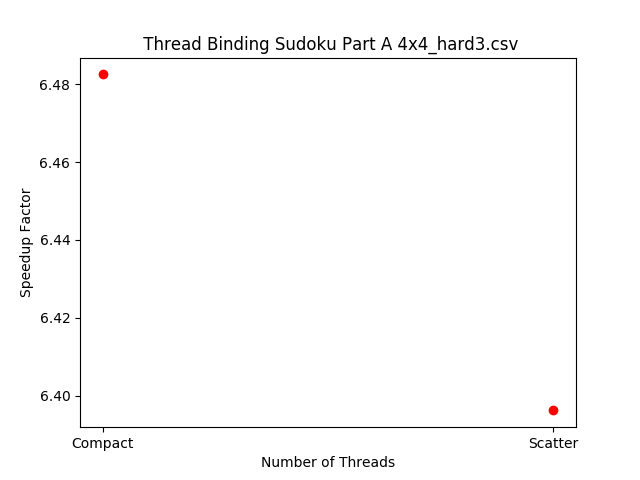
\includegraphics[width=1\linewidth]{./img/binding_part_2_A.png}
    \caption{Results for the blurring on strawberry image.}
\end{figure}

\newpage

\subsubsection{Part B}
\begin{description}
    \item[Different mapping strategies; Compact and Scatter]
\end{description}
\begin{figure}[!htb]
    \centering
    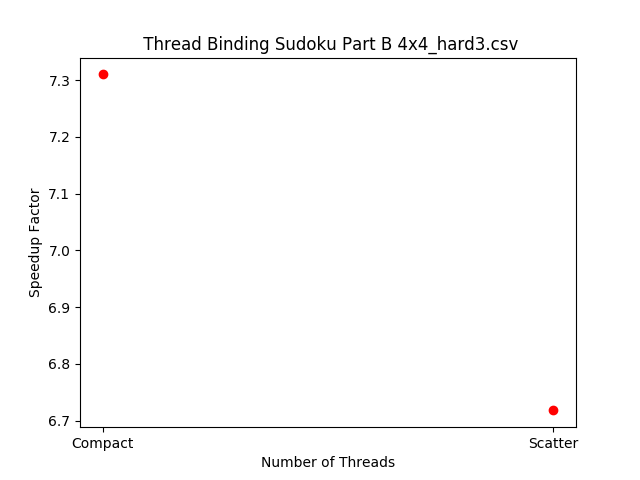
\includegraphics[width=1\linewidth]{./img/binding_part_2_B.png}
    \caption{Results for the blurring on strawberry image.}
\end{figure}

\newpage

\subsubsection{Part C}
\begin{description}
    \item[Different mapping strategies; Compact and Scatter]
\end{description}
\begin{figure}[!htb]
    \centering
    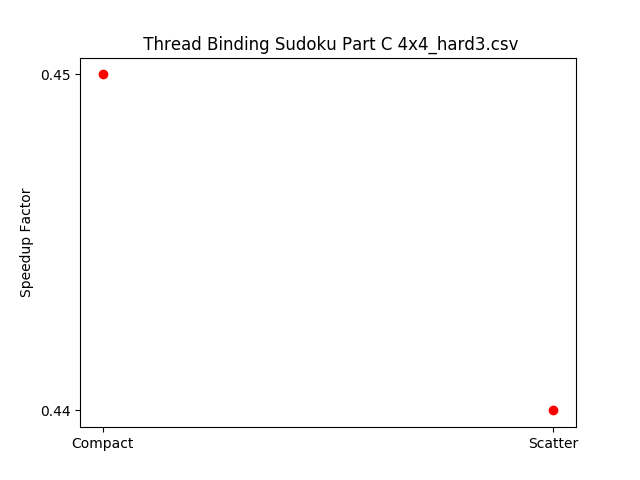
\includegraphics[width=1\linewidth]{./img/binding_part_2_C.png}
    \caption{Results for the blurring on strawberry image.}
\end{figure}

\newpage

\subsection{Tests on Sudoku Problems of Different Grids}
\begin{description}
\item[Part-B]
\end{description} 
\begin{figure}[!htb]
    \centering
    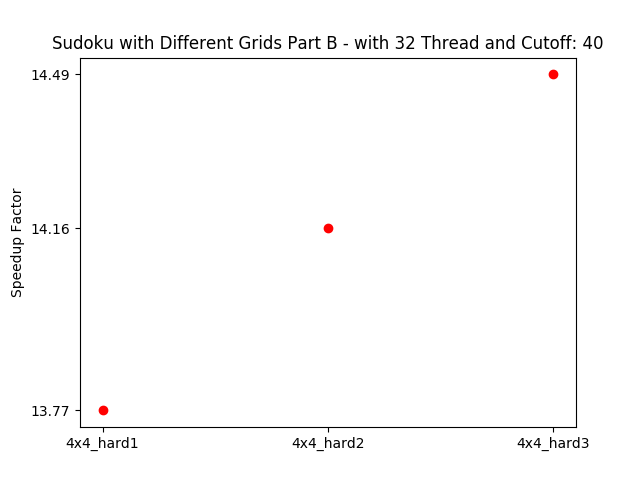
\includegraphics[width=1\linewidth]{./img/grids_part_2_B.png}
    \caption{Results for the 32 Thread Parallel Sudoku solver in Part with different sizes and difficulties.}
\end{figure}


%----------------------------------------------------------------------------------------
%	SECTION 6
%----------------------------------------------------------------------------------------

\section{Formulas Used}

\begin{enumerate}
\begin{item}
\emph{Speedup} 
\begin{equation*}
\frac{\mathrm{T1}}{\mathrm{Tp}}
\end{equation*}
\end{item}
\end{enumerate}




\end{document}